\section{Theoretical Analysis}
\label{sec:analysis}

In this section, the circuit shown in \textbf{Figure~\ref{fig:diagram_t5}} is analysed
theoretically.
\begin{figure}[h] \centering
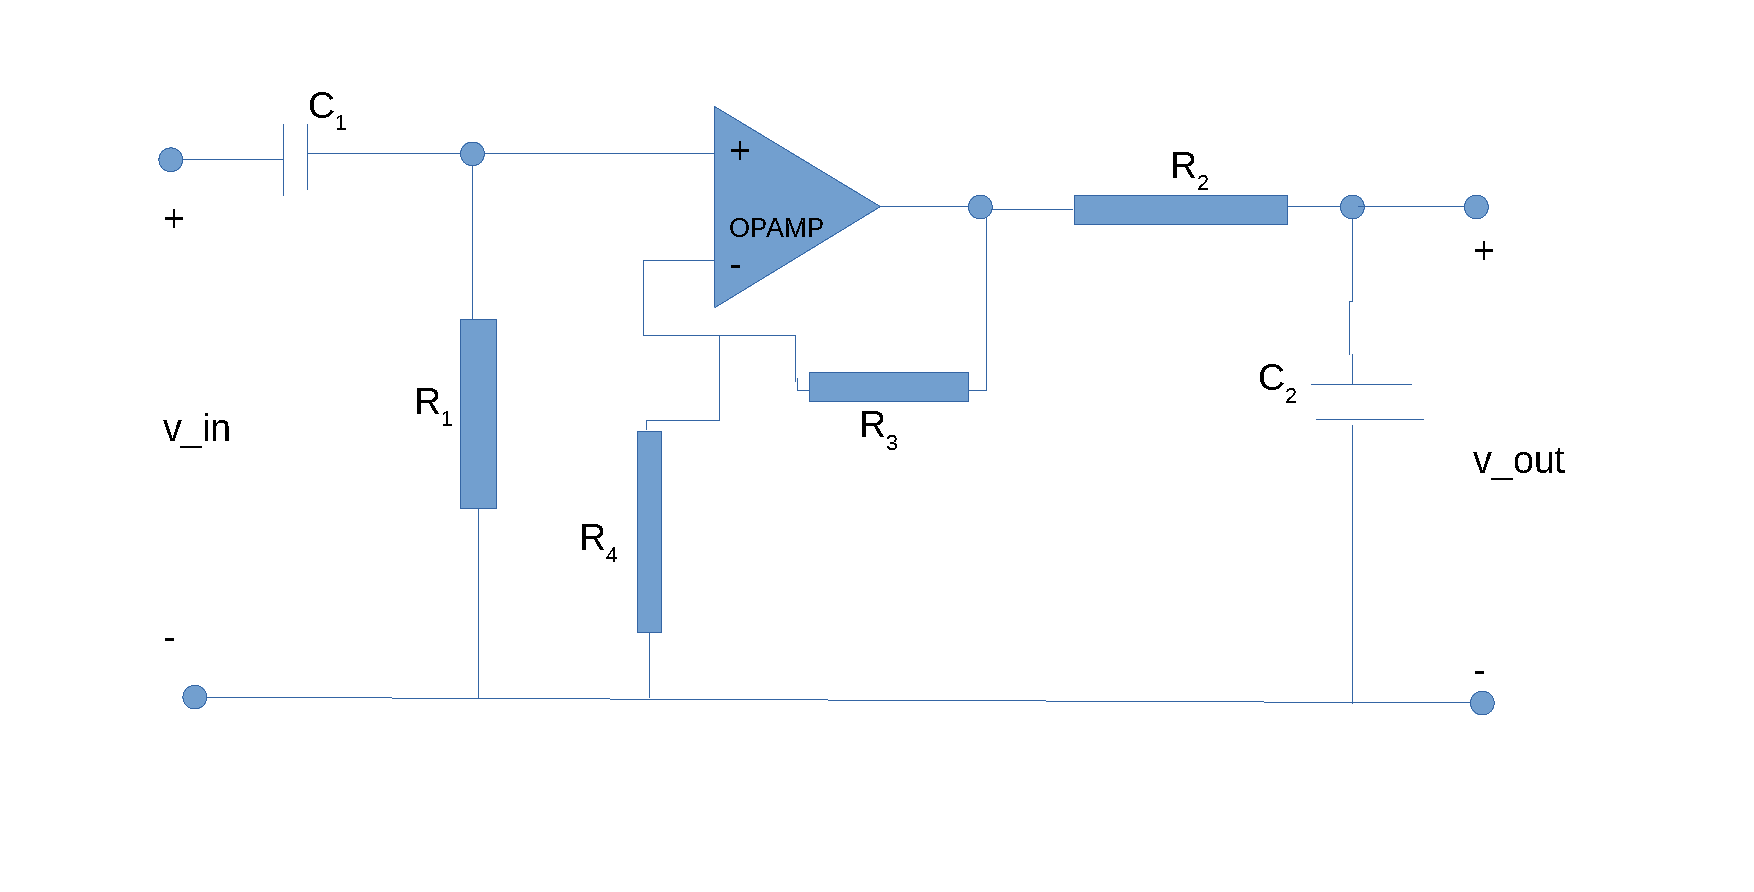
\includegraphics[width=0.95\linewidth]{diagram_t5.pdf}
%\vspace{-7cm}
\caption{Diagram of the circuit considered for the computations and simulations.}
\label{fig:diagram_t5}
\end{figure}


The objective of an OP-AMP BandPass filter (active bandpass filter) is to, as the name suggests, block unwanted frequencies, only allowing a certain bandwith of frequencies to pass through, whilst actively amplifing the signal for these frequencies. In this particular case we want the central frequency to be 1 KHz and the gain at this frequency to be 40 dB. This filter is a bit different from the one done in a previous lab, that only filtered the signal and did not amplify it (passive filter). For  a passive filter we would only need resistors and capacitors, but for an active filter we also need transistors or OP-Amps in order to amplify the signal. In this case we will use the 741 OP-AMP in an non inverting manner. At the same time, this circuit is also quite different from the previous lab assignment, where we just wanted to optimize a purpose-built audio amplifier (and had no intention of filtering the input signal).\par 


The lower cutoff frequency ($f_L = \frac{\omega_L}{2*\pi}$) for the circuit shown in \textbf{Figure~\ref{fig:diagram_t5}} will therefore be:
\begin {equation}
	f_L= \frac{1}{R_1*C_1*2*\pi}   
	\label{eq:lcf}
\end{equation}


and the upper cutoff frequency ($f_H = \frac{\omega_H}{2*\pi}$) is given by: 

\begin {equation}
	f_H = \frac{1}{R_2 *C_2* 2*\pi}  
	\label{eq:ucf}
\end{equation}

and thus the central angular frequency $\omega_O$ is determined by geometric centre of these, as such given by:

\begin {equation}
	\omega_O= \sqrt{\omega_L * \omega_H }  
	\label{eq:CentralF}
\end{equation}
 
the gain is given by:

\begin {equation}
	Gain= |\frac{R_1*C_1*\omega*j}{1+R_1*C_1*\omega*j}*(1+\frac{R_3}{R_4})*\frac{1}{1+R_2*C_2*\omega*j}|   	
	\label{eq:gain}
\end{equation} 
the transfer function is given by: 

\begin {equation}
	T(s) = \frac{R_1*C_1*s}{1+R_1*C_1*s}*(1+\frac{R_3}{R_4})*\frac{1}{1+R_2*C_2*s}   	
	\label{eq:gain}
\end{equation} 

and the input and output impedances are given by: 

\begin {equation}
	Z_{in} = R_1 + \frac{1}{j*\Omega_O*C_1} 
	\label{eq:impedances_in}
\end{equation}  

\begin {equation}
       Z_{out} = \frac{1}{j*\Omega_O*C_2+\frac{1}{R2}}	
	\label{eq:impedances_out}
\end{equation}  

A whiteboard image taken in the presential lab may help relate all these formulas:

\begin{figure}[h] \centering
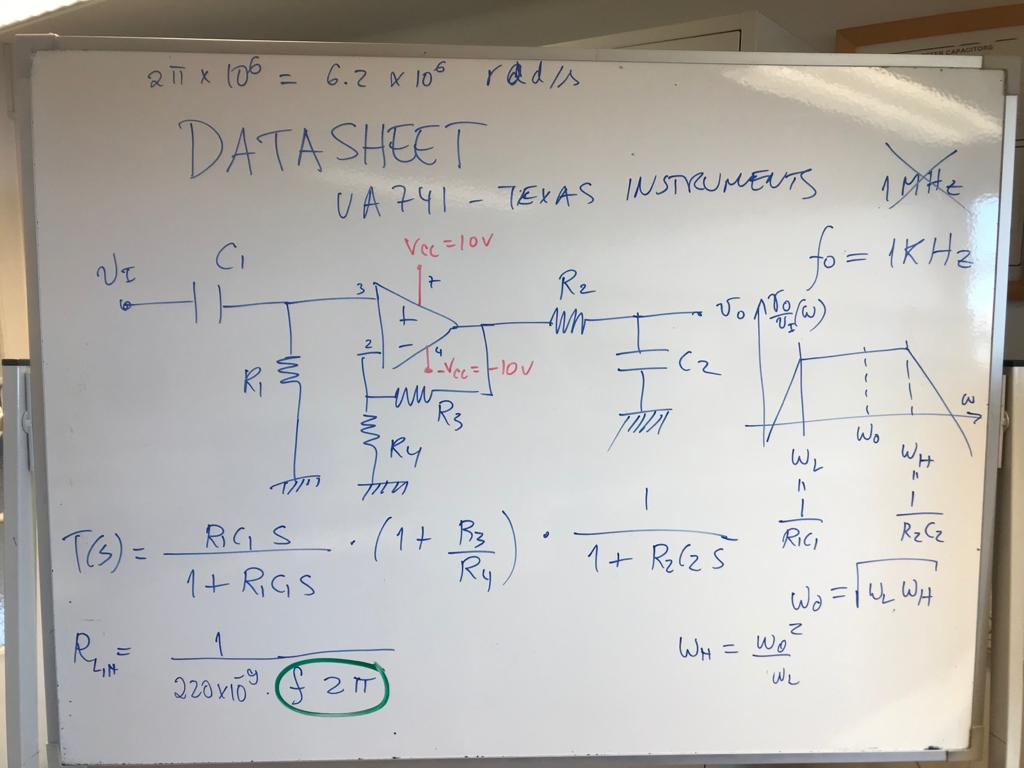
\includegraphics[width=0.95\linewidth]{datasheet.jpeg}
%\vspace{-7cm}
\caption{Sketch of the circuit and relevant formulas for its manipulation.}
\label{fig:formulas}
\end{figure}



With the materials available for this lab, the aid of the aforementioned formulas, some hand calculations (and through a little bit of trial and error), we arrived at the final values considered for the circuit parameters (as named in the above figure) that maximized the merit. These can be found in the following table. Do note that despite the available resistors being limited in quantity and value (only three of each of these types: 1$k\Omega$, 10$k\Omega$ and 100$k\Omega$), we were able to, combining these in parallels and in series, obtain a larger array of available equivalent resistor values (e.g. combining two 1$k\Omega$ in parallel yields a 500$\Omega$ resistor). This ability proved to be quite useful! In the case when intermediate resistor values are used (such as 5$k\Omega$ or 150$k\Omega$), the same sort of techniques were employed (using, respectively, two 10$k\Omega$ resistors in parrallel or three 100$k\Omega$ resistors, two in a parallel in series with the third).

\hfill
 \parbox{1\linewidth}{
  \centering
  \begin{tabular}{|l|l|r|}
    \hline    
    {\bf Parameter} & {\bf Value} & {\bf Units }\\ \hline
    \input{values.tex}
  \label{tab:params}
  \end{tabular}
  }
\par

In the following table the results (output voltage gain in the passband, the central frequency, and the input and output impedances at this frequency) for both for the theoretical analysis (right) and the Ngspice simulation (left) are presented in order to make a side-by-side comparison. The final cost and merit values are also included (do note that we also included the OPAMP cost in our cost calculations. This fixed value was computed by hand, by observation of the OPAMP model given to us in the Ngspice script, and yielded 1.3323e4 Monetary Units).\par
The circuit used for the theoretical calculations was the one schematized above. For the Ngspice simulations, this was also the main setup used, but a different setup was required to measure the outputd impedance. But we'll get there in the next section!\par
As can be easily noted, the theoretical and simulation results differ a lot. This is due mainly (as would be expected by now) to the fact that the OPAMP model used includes capacitors, which introduces, by means of additional complex impedances, two extra poles in the transfer function (this subverts the bode plots obtained by simulation and theoretically, as will be seen). This also affects the upper cutoff frequency, and, as a result, the central passband frequency: while, in theory, the parameters used will not give us the desired frequency (in fact it would be around 100Hz and not around 1kHz), in practice, they do! \par
At the same time, the output impedance values differ by several orders of magnitude, and the gain obtained via both methods is off by approximately 50\% (we focussed on the simulation values in this process, thinking of them as what we wished to optimize). In fact, the only similar values are the lower cutoff frequencies! (And, obviously, the cost is the same).\par
Due to all theses discrepancies, the merit figures are very different: the simulation merit is about 100x greater than the one obtained from the theoretical calculations. Even so, the merit figure is very low, in comparison with previous labs. We believe this is also a result of different characteristics of the circuits used (in particular, given the high, fixed and unavoidable cost of the OPAMP and the limited components, which make it hard to achieve low enough deviations, essential for a seemingly high merit figure). This goes to show us that, for complex components such as these, a bad model or an incomplete model is worse than no model at all!\par

\hfill
 \parbox{1\linewidth}{
  \centering
  \begin{tabular}{|l|l|l|r|}
    \hline    
    {\bf Parameter} & {\bf Simulation} & {\bf Theoretical } & {\bf Units }\\ \hline
    Zi & 766.402 & 640.49 & Ohm\\ \hline
Zo & 4.49605 & 2.9364 & Ohm\\ \hline
Cost & 8116 & Cost & MU\\ \hline
uco & 3106933.000 & 2123123123123.000 & Hz\\ \hline
lco & 7.924 & 2123123123123.000 & Hz\\ \hline
Bandwidth & 3106925.076 & 2123123123123.000 & Hz\\ \hline
Gainv(out) & 56.041 & -107.220 & [adimensional]\\ \hline
MERIT & 2707.5316 & -104.2260 & gold medals\\ \hline

  \label{tab:results}
  \end{tabular}
  }
  
  Note as well that uco and lco stand for, respectively, upper cutoff frequeny and lower cutoff frequency.
  The next figures present the frequency response obtained in the theoretical analysis.


\begin{figure}[H] \centering
\includegraphics[width=0.6\linewidth]{teo_gain.eps}
\caption{Output voltage gain frequency response of the BandPass Filter Amplifier. Note the plateau around 40dB (linear gain of 100) which occurs in the vicinity of 1kHz. This was the initial objective and this was as close as we could get with the available components.}
\label{fig:gain_octa}
\end{figure}

\begin{figure}[H] \centering
\includegraphics[width=0.6\linewidth]{teo_phase.eps}
\caption{Phase response of the BandPass Filter Amplifier.}
\label{fig:phase_octa}
\end{figure}



\pagebreak


